\documentclass[12pt,a4paper,openright,twoside]{book}
\usepackage[utf8]{inputenc}
\usepackage{disi-thesis}
\usepackage{code-lstlistings}
\usepackage{notes}
\usepackage{shortcuts}
\usepackage{acronym}
\usepackage{hyperref} % links
\usepackage{comment} % for multi-line comments
\usepackage{booktabs} % for better tables
\usepackage{xcolor}
\usepackage{listings}
\usepackage{caption}
\usepackage{subcaption}

\showboxdepth=5
\showboxbreadth=5

\school{\unibo}
\programme{Corso di Laurea Magistrale in Ingegneria e Scienze Informatiche}
\title{Fancy Title}
\author{Penazzi Paolo}
\date{\today}
\subject{Supervisor's course name}
\supervisor{Prof. Supervisor Here}
\cosupervisor{Prof. CoSupervisor 1}
\session{III}
\academicyear{2022-2023}

% Definition of acronyms
\acrodef{CAS}{Collective Adaptive System}
\acrodef{vm}[VM]{Virtual Machine}
\acrodef{SUT}{System Under Test}


\mainlinespacing{1.241} % line spacing in main matter, comment to default (1)

\begin{document}

\frontmatter\frontispiece

\begin{abstract}	
Max 2000 characters, strict.
\end{abstract}

%----------------------------------------------------------------------------------------
\tableofcontents   
\listoffigures     % (optional) comment if empty
\lstlistoflistings % (optional) comment if empty
%----------------------------------------------------------------------------------------

\mainmatter

%----------------------------------------------------------------------------------------
\chapter{Introduction}
\label{chap:introduction}
%----------------------------------------------------------------------------------------

% Testing
% Importance of Testing
% Benchamark
% Testing and Benchmarking in Computer Science
\paragraph*{Motivation}

\begin{comment}
  

In every field of engineering, testing is a fundamental part of the development process.
It is used to verify that the system meets the requirements and to assure that it has the desired quality.

A \textit{testbed} is a platform for experimentation and testing. 
It provides a rigorous, transparent and replicable environment for testing.
Testbed often makes use of simulators, which are software that allows the user to see how its program would behave in a real environment.

In computer science research, is important to evaluate the behavior of newly developed algorithms against state-of-the-art solutions.
This allows us to understand whether a newly developed solution is better than an existing one in a certain scenario.

To make this comparison \textit{benchmarks} are used. A benchmark is a reference against which a solution can be compared.

This work targets a specific category of systems, called \ac{CAS}.



We are interested in the different properties of these systems. Most of these can be measured by carrying out tests.

\end{comment}

\paragraph*{Objectives}

\paragraph*{Thesis Structure}

%----------------------------------------------------------------------------------------
\chapter{Background}
%----------------------------------------------------------------------------------------

\section{Collective Adaptive Systems}

Collective Adaptive Systems refer to a form of complex systems where a large number of heterogeneous entities interact without specific external or internal central control, 
adapt their behavior to environmental settings in pursuit of an individual or collective goal.
CAS often adopts cooperative operating strategies to run distributed decision-making mechanisms. \cite{DBLP:journals/tomacs/Aldini18}

A colony of ants is an example of CAS in nature: each ant is an autonomous entity that interacts with other ants and with the environment to achieve the common goal of the colony. 
Bird flocks, fish shoals, animal herds and human crowds are also examples of CAS.

These systems have been studied and modeled in different fields, such as computer science.
CASs have some interesting properties that make them suitable for many applications:

\begin{itemize}
  \item \textit{fault-tolerance} Each entity carries out a simple task, by doing so they are less prone to errors.
  \item \textit{scalability} Adding or removing an entity does not affect the system's behavior or performance.
  \item \textit{robustness} The failure of one or more entities does not affect the system's behavior or performance.
\end{itemize}

Drone swarms tasked with monitoring an area, wearable devices to manage crowd congestion during a public event, cars on streets connected to handle traffic, are all examples of artificial CAS. \cite{2}

\begin{figure*}[t]
  \centering
  \begin{subfigure}[b]{0.49\textwidth}
      \centering
      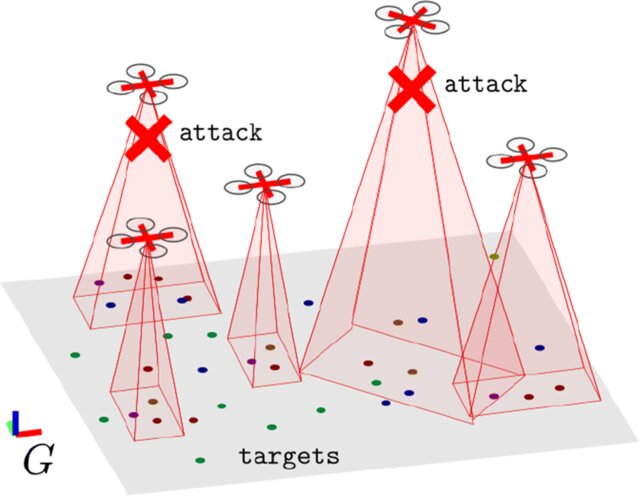
\includegraphics[width=0.9\textwidth]{figures/swarm2.jpeg}
  \end{subfigure}

  \begin{subfigure}[b]{0.49\textwidth}
      \centering
      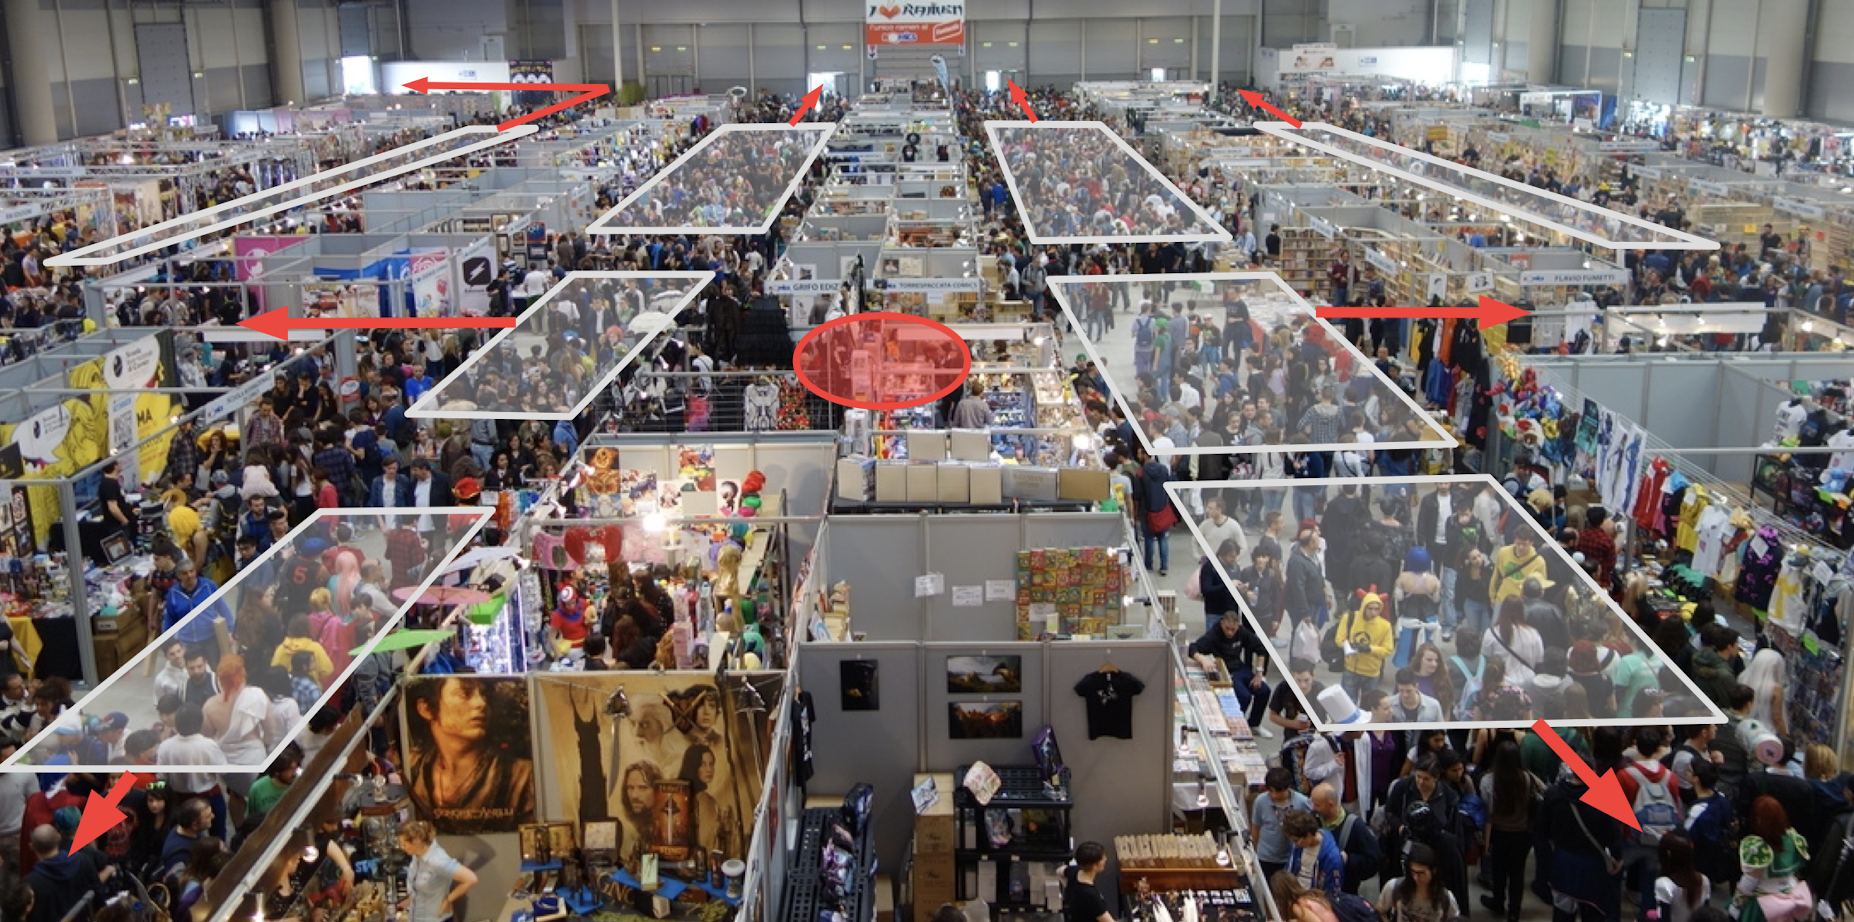
\includegraphics[width=0.8\textwidth]{figures/crowd.png}
  \end{subfigure}
  \caption{Some examples of CAS.}
\end{figure*}

\section{Aggregate Computing}

\section{Simulation}

In computer science, simulation is the process of executing software in a controlled environment to evaluate its behavior. 
Simulations can be used to test the correctness of a program, evaluate its performance, or understand its behavior in a specific scenario. 
The key point of a simulation is to execute the software under controlled and repeatable conditions to compare different executions. 
This cannot be done without a simulator, which is software that provides the user with all the tools needed to run the simulation. \cite{argun2021simulation, bagrodia1998parsec}

The importance of simulators and simulation becomes clear when testing CASs. 
It is not feasible to create a real environment, such as a network of 100 drones or a crowd of 1000 people, to test a program. 
Simulators allow us to create a virtual environment where we can run the program and evaluate its behavior.

The reference simulator for this work is Alchemist. \cite{Pianini_2013}

Alchemist is a meta-simulator for pervasive, aggregate, and nature-inspired computing. 

It supports different incarnations, such as Protelis, SAPERE and ScaFi. \cite{DBLP:conf/sac/PianiniVB15, DBLP:conf/saso/CastelliMRZ11, DBLP:journals/softx/CasadeiVAP22}


%----------------------------------------------------------------------------------------
\chapter{Domain Analysis}
%----------------------------------------------------------------------------------------

\begin{comment}
  STATE OF THE ART
  UBIQUITOUS LANGUAGE
  TECHNOLOGIES
      Containerization
      Language
\end{comment}

\section{Ubiquitous Language}

To better understand the problem domain and to avoid misunderstandings, a ubiquitous language was defined.

\begin{table}[h]
    \centering
    \begin{tabular}{|l|p{0.8\textwidth}|}
    \toprule
    \textbf{Term} & \textbf{Meaning} \\
    \midrule                                                                                                                                                              
    Testing & The overall process carried out to verify and validate a system, according to requirements, to promote the desired internal and external quality and to mitigate risks in development and products. \\ \hline
    Testbed & A platform for rigorous transparent and replicable environment for experimentation and testing TODO Cite \\ \hline
    Solution & A set of algorithms leading to achieving goals and overcoming the problem posted \\ \hline
    Scenario & Contains all the information about the test execution: the simulation platform, the metrics, the input parameters \\ \hline
    Program & TODO \\ \hline
    Simulator & A software that allows the user to see how its program would behave in a real environment \\ \hline
    Parser & Component of the Testbed responsible for the read of the input file \\ \hline
    Listener & Component of the Testbed responsible for the read of the output of the simulator \\ \hline
    \end{tabular}
    \caption{Domain Ubiquitous Language}
    \end{table}

\section{Technologies}

\subsection{Containerization}

% What is containerization
Containerization is a lightweight alternative to full-machine virtualization that involves encapsulating an application in a container with its operating environment.

% Why containerization is needed
The main reason for using containerization is to create a consistent, isolated environment for applications to run in.
By doing so, the user can be sure that the application will always run the same way, regardless of the user's machine configuration. 
Further, this allows the user to focus solely on the application itself, without having to worry about dependencies, software updates, compatibility and things like this.

% Choice of Docker as containerization technology
When choosing a containerization technology, the choice was between the two most popular solutions in this field: Docker and Kubernetes.
Ultimately, Docker was chosen because it is more lightweight and easier to use than Kubernetes.

% How Docker works
Docker is a platform for building, running, and shipping applications in containers.
Docker containers wrap up a piece of software in a complete filesystem that contains everything it needs to run:
code, runtime, system tools, system libraries - anything you can install on a server.
To create a container, a Dockerfile is needed, which is a text document that contains all the information to deploy the application.

\subsection{Language}
Different languages were considered for the implementation of the system.

\paragraph*{Scala}
Scala is a strong statically typed high-level general-purpose programming language that supports both object-oriented 
programming and functional programming. 
Designed to be concise, scalable and safe, many of Scala's design decisions are aimed at addressing criticisms of Java.
\cite{1}
One weakness of Scala is its steep learning curve, which makes it difficult to learn for new users.

\paragraph*{Kotlin}
Kotlin is a cross-platform, statically typed, general-purpose high-level programming language with type inference. 
Kotlin is designed to interoperate fully with Java.
Support for multiplatform programming is one of Kotlin’s key benefits. It reduces time spent writing and maintaining 
the same code for different platforms while retaining the flexibility and benefits of native programming.
%[https://github.com/JetBrains/kotlin]

\paragraph*{Rust}

Rust is a multi-paradigm programming language designed for performance and safety, especially safe concurrency. \\
It has been designed to be a safe, concurrent, practical language, supporting functional and imperative-procedural paradigms.
It is considered the modern version of C and C++.

\paragraph*{Final choice}
After a brief analysis, it was clear that both Kotlin and Scala were suitable candidates for the implementation of the system.
In the end, the choice fell on Kotlin.

%----------------------------------------------------------------------------------------
\chapter{Design}
%----------------------------------------------------------------------------------------

\section{Architecture}

\begin{figure}[h]
    \centering
    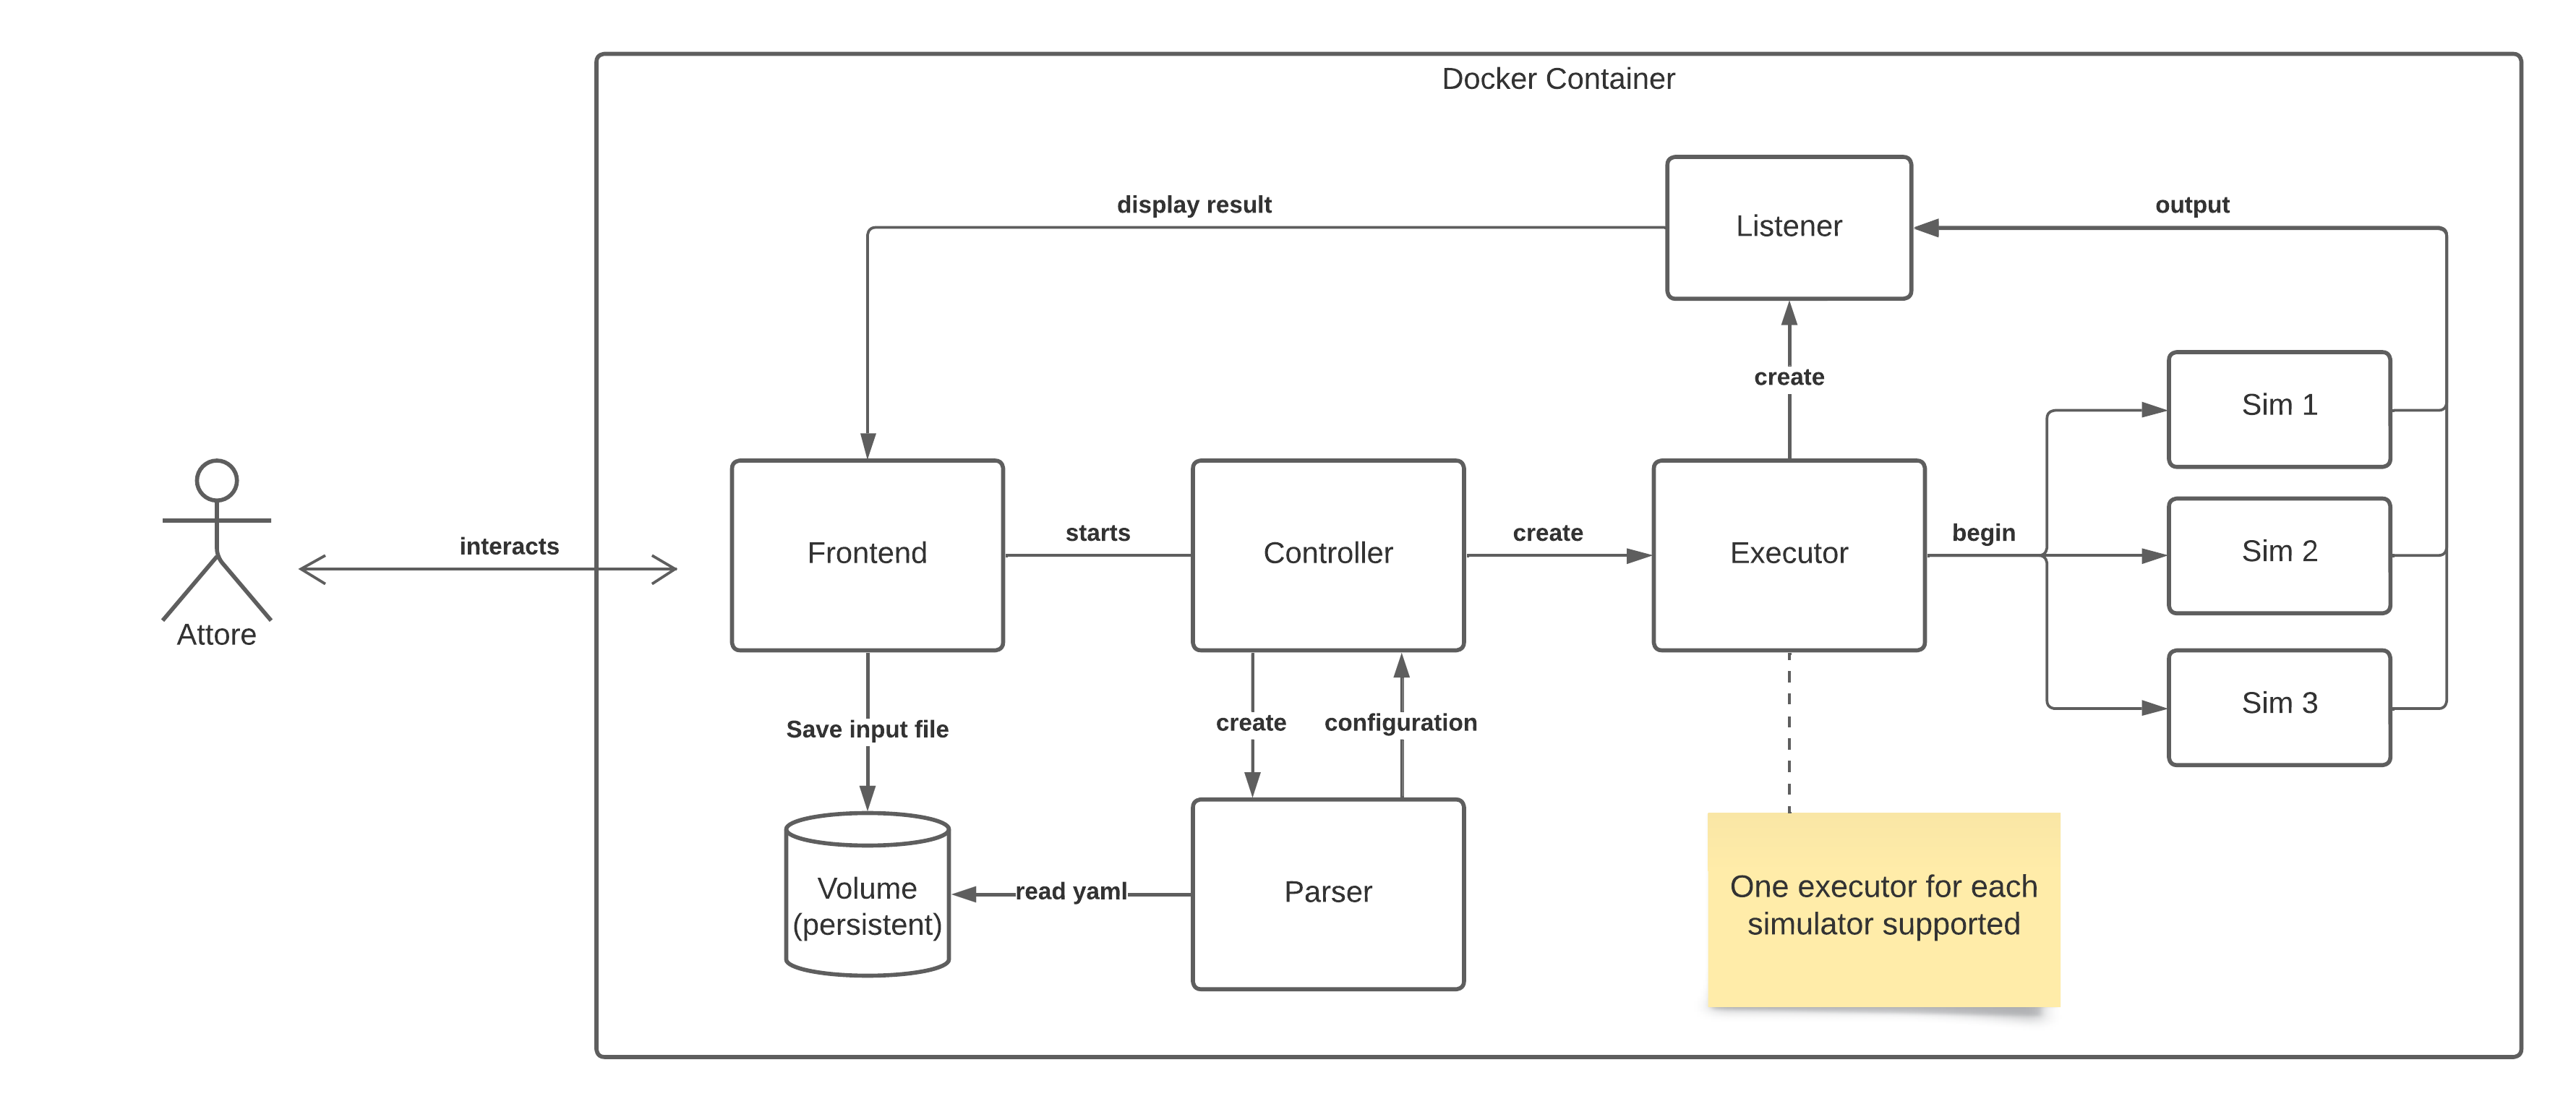
\includegraphics[width=\textwidth]{figures/architecture.png}
    \caption{Architecture of the system (v0.1)}
    \label{fig:random-image}
\end{figure}

\paragraph*{User Interaction} From an early analysis the better choice seems to be to deploy the framework online.
This means that the user doesn't have to install anything, but can use the framework by visiting the webpage.
(A step further would be using \href{https://kotlinlang.org/docs/multiplatform.html#kotlin-multiplatform-use-cases}{Kotlin Multiplatform} to deploy the framework for different platforms)

\paragraph*{Frontend} The frontend consists of a GUI that allows the user to interact with the software. 
A minimum interface has a button to load an input file (YAML), a button to start the simulation, and a box to show the results.

\paragraph*{Volume} A persistent data storage volume to keep all the input and output files in memory.

\paragraph*{Controller} When the user starts the simulation, it uses a parser to read the input file, create the simulation properties,
and starts the simulator-specific executor.

\subsection{Parser} 
The parser is responsible for reading the input file and creating the simulation model.

\paragraph*{Executor} The executor is responsible for the start of the simulation. It should be able to drive different simulators.

\paragraph*{Listener} The listener reads the output of the simulation and sends it to the GUI.
(In the image it is created by the executor but actually it may be the controller that creates the listener)

\subsection{Input Files}

One of the main challenges of this work is to create a flexible system that can be extended to support different simulators.
This means that the input file structure should take into account the possibility of being extended, without breaking the existing structure.

This is an input file example, which will be used to explain the structure of the input file.

\begin{lstlisting}[style=yaml]
strategy:
  multiThreaded: false
  executionOrder:
    - grid-random
    - grid-gradient

simulators:
  - name: Alchemist
    version: "28.0.1"
    scenarios:
      - name: grid
        description: A tutorial to Alchemist and Protelis incarnation
        scenarioConfiguration: "src/main/yaml/grid.yml"
        programs:
          - name: gradient
            description: A gradient program
            input: "src/main/yaml/gradient.yml"

          - name: random
            description: A random program
            input: "src/main/yaml/random.yml"
\end{lstlisting}

\paragraph*{Strategy} The strategy section contains generic information about the testbed configuration. None of these 
are simulator-specific instructions.
All the keywords in this section are optional, and if not specified the default value is used: the execution will be
single-threaded and the execution order will be random.

\paragraph*{Simulators} The simulators section contains the configuration of each simulator used in the testbed.
Each simulator has a name, a version, and a list of scenarios. The name is mandatory, while the version is optional 
and is currently not used. The testbed will always use the latest version.

The scenario configuration is more complex, as each simulator has different ways to configure the scenario.
When adding support for a new simulator, it is mandatory to specify how its configuration should be written in the input file.

At the moment, Alchemist is the only simulator officially supported by the testbed.
The Yaml file structure for Alchemist requires specifying a list of scenarios, each with a name, a description, and a path to the input file.
This input file contains all the information needed to run the simulation.

The user in some cases may want to run the same scenario with different programs.
To do so, the user can specify a scenario configuration and a list of programs, each with a name, a description, and a path to the input file.

The testbed will then generate a new Yaml file, by combining the scenario configuration and the program input file. 
The name of the generated file will be \textit{scenarioName-programName.yml}.

Here are some examples of input files for Alchemist.

\begin{lstlisting}[style=yaml, caption={Two programs to be tested in the same scenario}]
  simulators:
    - name: Alchemist
      version: "28.0.1"
      scenarios:
        - name: grid
          description: A tutorial to Alchemist and Protelis incarnation
          scenarioConfiguration: "src/main/yaml/grid.yml"
          programs:
            - name: gradient
              description: A gradient program
              input: "src/main/yaml/gradient.yml"
  
            - name: random
              description: A random program
              input: "src/main/yaml/random.yml"
  \end{lstlisting}

\begin{lstlisting}[style=yaml, caption={One scenario and one program. Both specified in the same input file.}]
- name: Alchemist
  version: "28.0.1"
  scenarios:
    - name: Alchemist-Sapere
      description: A tutorial to Alchemist and Sapere incarnation
      input: "src/main/yaml/tutorial.yml"
\end{lstlisting}

\subsection{Model}
The testbed model should follow the input file structure. 
This allows the Parser to convert the YAML file directly into the testbed model.

\begin{figure}[h]
  \centering
  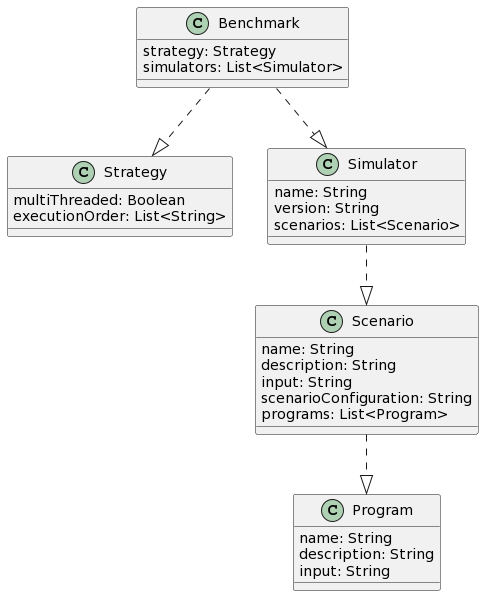
\includegraphics[width=0.7\textwidth]{figures/model.png}
  \caption{Model of the system (v0.1)}
  \label{fig:model}
\end{figure}

As can be seen from the image, the model is 1:1 with the input file.

%----------------------------------------------------------------------------------------
\chapter{Implementation}
%----------------------------------------------------------------------------------------

%----------------------------------------------------------------------------------------
\chapter{Evaluation}
%----------------------------------------------------------------------------------------

%----------------------------------------------------------------------------------------
\chapter{Conclusion and Future Work}
%----------------------------------------------------------------------------------------

%----------------------------------------------------------------------------------------
% BIBLIOGRAPHY
%----------------------------------------------------------------------------------------

\backmatter

%\nocite{*} % comment this to only show the referenced entries from the .bib file

\bibliographystyle{plain}
\bibliography{bibliography}

\end{document}
